\chapter{Dalle CNN alle Graph Neural Networks}
\label{ch:from-cnn-to-gnn}

\section{Reti neurali e convoluzione su griglia: cosa si perde su un grafo}
\label{sec:neural-networks-classical-convolution-recap}

Il \Cref{ch:mathematical-foundations} ha costruito l'apparato matematico necessario a definire un filtro su un grafo, che si traduce ora in un modello che apprende dai dati. Il punto di partenza è il modello neurale più semplice, il percettrone multistrato (\emph{multilayer perceptron}, MLP), che rappresenta l'input come un vettore $h^{(0)}\in\mathbb{R}^{F_0}$ e lo trasforma applicando in sequenza $L$ strati della forma
\begin{equation}
\label{eq:mlp-layer}
h^{(l+1)} = \sigma\!\left(W^{(l)}h^{(l)} + b^{(l)}\right),
\end{equation}
dove $W^{(l)}\in\mathbb{R}^{F_{l+1}\times F_l}$ e $b^{(l)}\in\mathbb{R}^{F_{l+1}}$ sono i parametri appresi\footnote{Si segnala una collisione di notazione: nel \Cref{ch:mathematical-foundations} il simbolo $W$ denota la matrice dei pesi del grafo. $W^{(l)}$ denota invece la matrice dei parametri appresi dallo strato $l$ nelle reti neurali. Nel seguito la distinzione è affidata all'apice: $W$ resta la matrice dei pesi del grafo, $W^{(l)}$ è sempre una matrice di parametri.} e $\sigma$ è una funzione non lineare applicata componente per componente — tipicamente $\mathrm{ReLU}(z)=\max(0,z)$ negli strati interni, oppure sigmoide o tangente iperbolica quando l'uscita va vincolata a un intervallo limitato. La non linearità è essenziale: componendo strati puramente lineari si otterrebbe ancora una trasformazione lineare, e la profondità non aggiungerebbe alcuna capacità espressiva~\cite{goodfellow2016deep}.

I parametri si stimano minimizzando una funzione di perdita tramite discesa del gradiente. Il gradiente rispetto a ciascun $W^{(l)}$ si calcola con la \emph{backpropagation}~\cite{rumelhart1986learning}, ovvero l'applicazione sistematica della regola della catena percorrendo all'indietro il grafo delle operazioni, in modo da riusare i risultati parziali già calcolati invece di ricalcolarli per ogni parametro\footnote{Il costo di una passata di backpropagation è dello stesso ordine di quello della passata in avanti: è questa proprietà, e non la formula in sé, a rendere praticabile l'addestramento di reti profonde.}. Il meccanismo di addestramento resta lo stesso per tutte le architetture discusse nel seguito: cambia solo la forma dello strato, cioè l'equazione~\eqref{eq:mlp-layer}.

\subsection{Le proprietà della convoluzione su griglia}

Si consideri ora un input che, a differenza del vettore generico $h^{(0)}$ dell'MLP, possiede una struttura nota, come un'immagine: una griglia bidimensionale di pixel dotata di una nozione di vicinanza spaziale. Applicare direttamente l'equazione~\eqref{eq:mlp-layer} a tale input, appiattendolo in un vettore, è possibile ma disastroso: il numero di parametri cresce con il prodotto delle dimensioni dell'input e del layer, e ogni pixel viene trattato come una coordinata indipendente, senza alcuna nozione di vicinanza spaziale. La rete convoluzionale (\emph{convolutional neural network}, CNN) sostituisce il prodotto matrice-vettore denso con una convoluzione discreta~\cite{lecun1998gradient}, che nel caso monodimensionale si scrive:
\begin{equation}
\label{eq:discrete-convolution}
(x \ast k)[n] = \sum_{m} x[n-m]\,k[m],
\end{equation}
dove il filtro $k$ ha supporto limitato a poche posizioni attorno all'origine. Da questa scrittura discendono le seguenti tre proprietà:

\begin{description}
    \item[Località.] L'uscita in posizione $n$ dipende solo dai valori di $x$ in un intorno di $n$ ampio quanto il supporto di $k$. La struttura del dominio dice quali variabili possono interagire e a quale distanza.
    \item[Condivisione dei pesi.] Lo stesso vettore $k$ è usato in tutte le posizioni $n$: il numero di parametri dipende dall'ampiezza del filtro, non dalla dimensione dell'input. Un filtro $3\times3$ ha nove pesi tanto su un'immagine $32\times32$ quanto su una $4000\times3000$.
    \item[Equivarianza per traslazione.] Se l'input viene traslato, l'uscita si trasla della stessa quantità. Un \emph{pattern} riconosciuto in un punto dell'immagine è riconosciuto ovunque, senza doverlo riapprendere.
\end{description}

Nessuna delle tre proprietà sopravvive al passaggio a un grafo, e il motivo è strutturale piuttosto che tecnico. La formula~\eqref{eq:discrete-convolution} presuppone che le posizioni $n$ e $m$ vivano in un insieme dotato di un'operazione di somma: è la griglia, con la sua struttura di gruppo, a dare senso alla scrittura $n-m$. Su un grafo generico questa struttura non esiste: non è disponibile, in particolare, alcuna operazione che sposti un nodo in un altro preservando l'intera struttura di adiacenza, cioè l'azione di gruppo rispetto a cui l'equivarianza per traslazione dovrebbe essere definita. Viene meno, per la stessa ragione, anche il criterio su cui si fonda la condivisione dei pesi: senza un'operazione di traslazione, due punti del dominio non sono confrontabili come \enquote{la stessa posizione}, e non è quindi definibile se lo stesso filtro venga riusato in punti diversi. Sulla griglia, l'equivarianza per traslazione garantiva l'indipendenza dell'operatore dall'etichetta arbitraria assegnata a ciascuna posizione. Sul grafo questa proprietà dovrà essere recuperata in un'altra forma, ovvero come invarianza rispetto all'ordine, anch'esso arbitrario, in cui i nodi vengono elencati.

Ancora più concreto è il problema dell'ordinamento dei vicini. In una griglia ogni pixel ha esattamente otto vicini e ciascuno occupa una posizione identificabile che permette di assegnargli il peso corrispondente in $k$. Su un grafo, i vicini di un nodo formano un insieme: non sono numerati e la numerazione $v_1,\dots,v_N$ introdotta nella \cref{def:weighted-graph} è arbitraria, frutto dell'ordine in cui i nodi sono stati elencati e non di una loro proprietà. Inoltre, due nodi diversi hanno in generale un numero diverso di vicini, per cui un filtro a dimensione fissa non avrebbe nemmeno una forma ben definita.

\begin{figure}[t]
\centering
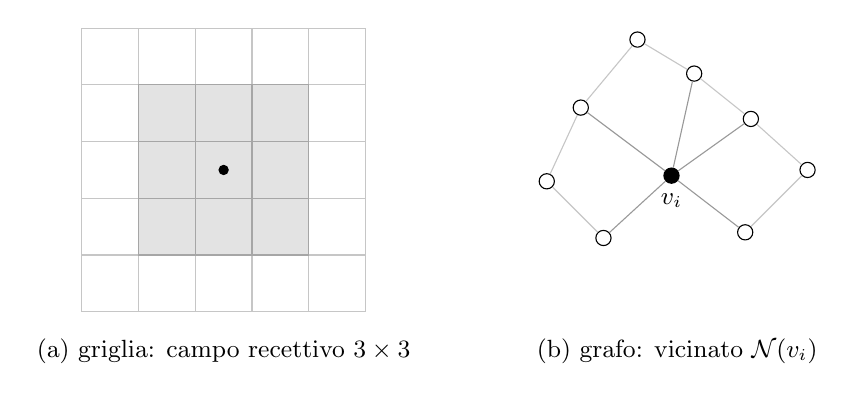
\begin{tikzpicture}[scale=0.72, every node/.style={font=\small}]
% --- griglia ---
\begin{scope}
    \foreach \i in {0,...,4} {
        \foreach \j in {0,...,4} {
            \draw[gray!45] (\i,\j) rectangle ++(1,1);
        }
    }
    \fill[gray!22] (1,1) rectangle (4,4);
    \foreach \i in {1,2,3} {
        \foreach \j in {1,2,3} {
            \draw[gray!70] (\i,\j) rectangle ++(1,1);
        }
    }
    \fill[black] (2.5,2.5) circle (2.6pt);
    \node at (2.5,-0.7) {(a) griglia: campo recettivo $3\times3$};
\end{scope}
% --- grafo ---
\begin{scope}[xshift=8.2cm, yshift=0.3cm]
    \tikzset{nd/.style={circle, draw, inner sep=0pt, minimum size=5.5pt, fill=white}}
    \node[nd, fill=black, label=below:{$v_i$}] (c) at (2.2,2.1) {};
    \node[nd] (a1) at (0.6,3.3) {};
    \node[nd] (a2) at (1.0,1.0) {};
    \node[nd] (a3) at (3.6,3.1) {};
    \node[nd] (a4) at (3.5,1.1) {};
    \node[nd] (a5) at (2.6,3.9) {};
    \node[nd] (b1) at (0.0,2.0) {};
    \node[nd] (b2) at (4.6,2.2) {};
    \node[nd] (b3) at (1.6,4.5) {};
    \draw[gray!80] (c)--(a1) (c)--(a2) (c)--(a3) (c)--(a4) (c)--(a5);
    \draw[gray!45] (a1)--(b1) (a2)--(b1) (a3)--(b2) (a4)--(b2) (a5)--(b3) (a1)--(b3) (a3)--(a5);
    \node at (2.3,-1.0) {(b) grafo: vicinato $\mathcal{N}(v_i)$};
\end{scope}
\end{tikzpicture}
\caption[Campo recettivo su griglia e vicinato su grafo]{Confronto tra il campo recettivo di un filtro convoluzionale su griglia e il vicinato di un nodo su un grafo. A sinistra ogni posizione del filtro è identificata dallo spostamento rispetto al pixel centrale e lo stesso filtro scorre su tutta l'immagine. A destra i vicini del nodo $v_i$ formano un insieme non ordinato e di cardinalità variabile da nodo a nodo: non esiste una posizione \enquote{in alto a destra} a cui associare un peso.}
\label{fig:grid-vs-graph}
\end{figure}

La \Cref{fig:grid-vs-graph} riassume il confronto. L'operazione di aggregazione sui vicini deve allora essere una funzione \emph{simmetrica} dell'insieme dei vicini, cioè invariante rispetto all'ordine in cui questi vengono elencati. Un'architettura che non rispetti questo vincolo produrrebbe uscite diverse a seconda di come si è scelto di numerare i nodi, e la numerazione non è un dato del problema. In termini più generali, il modello deve essere \emph{equivariante per permutazione}: permutare i nodi in ingresso deve permutare allo stesso modo le rappresentazioni in uscita, senza alterarle~\cite{bronstein2021geometric}.

Il \Cref{ch:mathematical-foundations} ha già indicato la soluzione a questo problema. Se la convoluzione non si può definire per traslazione nel dominio dei nodi, la si può definire nel dominio spettrale: la \cref{sec:graph-signal-processing-fourier} ha mostrato che l'operazione $g\ast_G x = Ug(\Lambda)U^\top x$ è la trasposizione sul grafo del teorema di convoluzione classico e che quindi una nozione di frequenza — e con essa di filtraggio — esiste anche in assenza di griglia.

\section{Approcci spettrali}
\label{sec:spectral-cnn-chebnet}

\subsection{Prima generazione: filtri liberi nel dominio spettrale}

Il primo tentativo di rendere operativa questa idea è quello del matematico Bruna et al.~\cite{bruna2014spectral}. La loro proposta è la traduzione più diretta possibile della \cref{sec:graph-signal-processing-fourier} in un layer addestrabile. Se un filtro su grafo è una funzione applicata allo spettro del Laplaciano, allora è possibile parametrizzare direttamente quella funzione, lasciando che sia la discesa del gradiente a sceglierne i valori. Il filtro diventa un vettore di parametri liberi $\theta=(\theta_1,\dots,\theta_N)\in\mathbb{R}^N$, uno per autovalore, e il layer si scrive:
\begin{equation}
\label{eq:spectral-cnn}
y = U\,\mathrm{diag}(\theta)\,U^\top x,
\end{equation}
con $U$ la matrice degli autovettori del Laplaciano introdotta nel \cref{thm:spectral-decomposition}.

L'interpretazione è trasparente: $U^\top x$ porta il segnale nel dominio delle frequenze del grafo, $\mathrm{diag}(\theta)$ amplifica o attenua ciascun modo, $U$ riporta il risultato sui nodi. Formalmente è una convoluzione su grafo a tutti gli effetti, ed è equivariante per permutazione come richiesto nella \cref{sec:neural-networks-classical-convolution-recap}. Nella pratica, però, presenta tre difetti principali.

Il primo è il numero di parametri. Un filtro ha $N$ gradi di libertà, uno per ogni nodo del grafo. La condivisione dei pesi della \cref{sec:neural-networks-classical-convolution-recap} è dunque persa e il modello cresce con la dimensione del dominio, esattamente come l'MLP applicato all'immagine appiattita.

Più gravemente, i parametri sono legati ad un particolare $U$, quindi ad un particolare grafo: un filtro appreso su un grafo non può essere trasferito ad un altro, neanche se ha lo stesso numero di nodi del primo. Nel caso del grafo delle criptovalute, ricalcolato a ogni finestra temporale (\cref{sec:dynamic-graphs-temporal-question}), questa è una limitazione cruciale.

Il secondo difetto è l'assenza di localizzazione. L'equazione~\eqref{eq:spectral-cnn} non impone che l'uscita sul nodo $i$ dipenda solo dai nodi vicini: per un $\theta$ arbitrario la matrice $U\,\mathrm{diag}(\theta)\,U^\top$ è densa, perché gli autovettori del Laplaciano hanno in generale supporto sull'intero grafo. L'analogo dell'ampiezza del filtro convoluzionale — la prima delle tre proprietà della \cref{sec:neural-networks-classical-convolution-recap} — non è controllabile.

Il terzo è computazionale: l'equazione~\eqref{eq:spectral-cnn} richiede $U$, cioè la decomposizione spettrale completa del Laplaciano, che la \cref{sec:computational-aspects-sparse-eigensolvers} ha quantificato in $O(N^3)$ operazioni, a cui si aggiunge un costo $O(N^2)$ per ogni applicazione del filtro (due prodotti matrice-vettore densi). Su un grafo di poche decine di criptovalute il conto è indolore; sui grafi con milioni di nodi è proibitivo.

\subsection{Filtri polinomiali}

I tre difetti hanno una radice comune: $\theta$ è una funzione arbitraria degli autovalori, definita punto per punto. Li si affronta tutti insieme imponendo che il filtro sia un \emph{polinomio} dello spettro:
\begin{equation}
\label{eq:polynomial-filter}
g_\theta(\Lambda) = \sum_{k=0}^{K}\theta_k\Lambda^k, \qquad \theta \in \mathbb{R}^{K+1}.
\end{equation}
Il numero di parametri scende da $N$ a $K+1$, indipendente dalla dimensione del grafo. Il vincolo restituisce inoltre gratuitamente la località, e con essa la possibilità di fare a meno di $U$. Entrambe le conseguenze discendono da un'unica osservazione algebrica.

\begin{proposition}[Località delle potenze del Laplaciano]
\label{prop:laplacian-powers-locality}
Sia $d_G(i,j)$ la distanza sul grafo tra $v_i$ e $v_j$, cioè il numero minimo di archi di un cammino che li collega. Allora, per ogni $k\geq0$,
$$d_G(i,j) > k \implies (L^k)_{ij} = 0.$$
\end{proposition}

\begin{proof}
Per induzione su $k$. Per $k=0$, $L^0=I$: se $d_G(i,j)>0$ allora $i\neq j$ e $I_{ij}=0$. Per $k=1$, $L=D-W$ è nulla fuori dalla diagonale e dagli archi, quindi $l_{ij}=0$ non appena $d_G(i,j)>1$.

Si supponga ora l'enunciato vero per $k-1$ e siano $i,j$ con $d_G(i,j)>k$. Scrivendo $(L^k)_{ij}=\sum_m (L^{k-1})_{im}l_{mj}$, si osserva che ogni addendo è nullo: se $l_{mj}\neq0$ allora $d_G(m,j)\leq1$, e per la disuguaglianza triangolare $d_G(i,m)\geq d_G(i,j)-d_G(m,j) > k-1$, per cui $(L^{k-1})_{im}=0$ per ipotesi induttiva. La somma è dunque nulla. \qedhere
\end{proof}

Questa proposizione ha una conseguenza immediata per la quale ChebNet e la Graph Convolutional Network adottano proprio questa parametrizzazione polinomiale. Applicando il filtro polinomiale nel dominio dei nodi:
\begin{equation}
\label{eq:polynomial-filter-nodes}
U g_\theta(\Lambda)U^\top = \sum_{k=0}^{K}\theta_k\,U\Lambda^kU^\top = \sum_{k=0}^{K}\theta_k L^k.
\end{equation}
L'ultimo passaggio usa $U\Lambda^kU^\top = (U\Lambda U^\top)^k = L^k$, valida perché $U^\top U=I$ fa collassare i fattori intermedi. Per la \cref{prop:laplacian-powers-locality}, l'entrata $(i,j)$ della matrice risultante è nulla appena $d_G(i,j)>K$: un filtro polinomiale di grado $K$ è esattamente $K$-localizzato, cioè l'uscita su un nodo dipende solo dai nodi raggiungibili in al più $K$ passi. La località, che nella CNN era imposta a mano scegliendo l'ampiezza del filtro, qui è una conseguenza dimostrata del grado del polinomio.

Il secondo guadagno è racchiuso nell'equazione~\eqref{eq:polynomial-filter-nodes} stessa: il membro di destra non contiene più $U$. Gli autovettori sono serviti a definire l'operazione e a giustificarne il significato spettrale, ma spariscono dalla formula operativa, che richiede soltanto potenze di $L$. Poiché $L$ è sparso, il prodotto $Lx$ costa $O(|E|)$ (\cref{sec:computational-aspects-sparse-eigensolvers}), e applicare il filtro si riduce a $K$ prodotti matrice-vettore in cascata: $O(K|E|)$ contro $O(N^3)$, senza mai calcolare un autovettore.

\subsection{ChebNet}

Il vincolo che ha appena risolto i tre difetti della Spectral CNN introduce però un problema nuovo, di natura numerica. La base monomiale $\{1,\Lambda,\Lambda^2,\dots\}$ dell'equazione~\eqref{eq:polynomial-filter} è mal condizionata: al crescere di $k$ le potenze $\lambda^k$ diventano quasi indistinguibili tra loro sull'intervallo di interesse e i coefficienti $\theta_k$ diventano fortemente correlati e l'ottimizzazione ne risente. Defferrard et al.~\cite{defferrard2016chebnet} sostituiscono quindi i monomi con i polinomi di Chebyshev di prima specie, definiti dalla ricorsione
\begin{equation}
\label{eq:chebyshev-recursion}
T_0(x)=1,\qquad T_1(x)=x,\qquad T_k(x)=2x\,T_{k-1}(x)-T_{k-2}(x),
\end{equation}
che sull'intervallo $[-1,1]$ formano una base ortogonale\footnote{Ortogonale rispetto al prodotto scalare pesato $\langle f,g\rangle=\int_{-1}^{1}f(x)g(x)(1-x^2)^{-1/2}\mathrm{d}x$. La proprietà rilevante è che, a differenza dei monomi, i $T_k$ restano ben distinguibili tra loro al crescere del grado, e oscillano in $[-1,1]$ senza esplodere. Segue la stabilità numerica dell'approssimazione.} e godono di buone proprietà di approssimazione. Poiché i $T_k$ sono definiti su $[-1,1]$ mentre lo spettro di $L$ vive in $[0,\lambda_{\max}]$, il Laplaciano va riscalato:
\begin{equation}
\label{eq:laplacian-rescaled}
\tilde L = \frac{2}{\lambda_{\max}}L - I,
\end{equation}
trasformazione affine che manda $[0,\lambda_{\max}]$ in $[-1,1]$. Il layer ChebNet è allora
\begin{equation}
\label{eq:chebnet}
y = g_\theta(\tilde L)\,x = \sum_{k=0}^{K}\theta_k\,T_k(\tilde L)\,x .
\end{equation}

Il calcolo non richiede di costruire esplicitamente le matrici $T_k(\tilde L)$. Posto $\bar x_k = T_k(\tilde L)x$, la ricorsione~\eqref{eq:chebyshev-recursion} applicata a $\tilde L$ e valutata su $x$ dà
$$\bar x_0 = x,\qquad \bar x_1 = \tilde Lx,\qquad \bar x_k = 2\tilde L\bar x_{k-1}-\bar x_{k-2},$$
cioè una successione di vettori, ciascuno ottenuto dai due precedenti con un solo prodotto matrice-vettore sparso; l'uscita è la combinazione lineare $\sum_k\theta_k\bar x_k$. Il costo complessivo è $O(K|E|)$ e la memoria richiesta è quella di tre vettori alla volta, non di $K$ matrici $N\times N$.

Il bilancio rispetto all'equazione~\eqref{eq:spectral-cnn} è netto su tutti e tre i fronti: $K+1$ parametri indipendenti da $N$ e trasferibili tra grafi diversi, localizzazione a $K$ passi garantita dalla \cref{prop:laplacian-powers-locality}, nessuna decomposizione spettrale\footnote{Sopravvive una sola dipendenza spettrale, il valore $\lambda_{\max}$ nell'equazione~\eqref{eq:laplacian-rescaled}. Non serve però l'intera decomposizione: basta il solo autovalore massimo, ottenibile con i metodi iterativi della \cref{sec:computational-aspects-sparse-eigensolvers}.}. Restano due parametri liberi da fissare: $K$ e la scelta di normalizzazione del Laplaciano. È proprio spingendo all'estremo la prima scelta che si ottiene la Graph Convolutional Network.

\section{La Graph Convolutional Network}
\label{sec:gcn-kipf-welling}

L'architettura della Graph Convolutional Network nasce dal tentativo di semplificare il più possibile l'equazione~\eqref{eq:chebnet} senza perderne le proprietà essenziali. La risposta di Kipf e Welling~\cite{kipf2017gcn} è che si può arrivare fino a $K=1$ — un filtro che guarda i soli vicini immediati — a patto di compensare la perdita di espressività con la profondità, impilando più layer invece di allargarne uno solo. La derivazione procede nei seguenti tre passi.

\paragraph{Primo passo: $K=1$.} Ponendo $K=1$ nell'equazione~\eqref{eq:chebnet}, con $T_0(\tilde L)=I$ e $T_1(\tilde L)=\tilde L$, si ottiene
\begin{equation}
\label{eq:gcn-step1}
y = \theta_0 x + \theta_1\tilde Lx = \theta_0x + \theta_1\!\left(\frac{2}{\lambda_{\max}}L_{\mathrm{sym}} - I\right)\!x,
\end{equation}
dove si è scelto di lavorare con il Laplaciano normalizzato simmetrico $L_{\mathrm{sym}}$ della \cref{def:laplacian} anziché con il combinatorio: la normalizzazione, come discusso nella \cref{sec:graph-laplacian}, evita che i nodi ad alto grado dominino l'operatore.

\paragraph{Secondo passo: $\lambda_{\max}\approx2$.} Per $L_{\mathrm{sym}}$ vale $\lambda_{\max}\leq2$, con uguaglianza se e solo se il grafo ha una componente connessa bipartita\footnote{Un grafo è bipartito se i suoi nodi si possono partizionare in due insiemi tali che ogni arco colleghi un insieme all'altro. Il caso è improbabile in un grafo di correlazione tra criptovalute, in cui ogni asset tende a essere connesso a molti altri. Si può assumere $\lambda_{\max}$ prossimo a $2$ senza commettere un errore rilevante.}. Approssimando $\lambda_{\max}\approx2$, il fattore di riscalatura $2/\lambda_{\max}$ diventa $1$ e l'equazione~\eqref{eq:gcn-step1} si riduce a
$$y = \theta_0x + \theta_1(L_{\mathrm{sym}}-I)x = \theta_0x - \theta_1 D^{-1/2}WD^{-1/2}x,$$
avendo usato $L_{\mathrm{sym}} = I - D^{-1/2}WD^{-1/2}$. L'approssimazione elimina l'ultima dipendenza spettrale residua segnalata nella \cref{sec:spectral-cnn-chebnet}: non compare più alcun autovalore, e il modello non ha bisogno di alcun calcolo spettrale.

\paragraph{Terzo passo: un solo parametro.} I due coefficienti $\theta_0$ e $\theta_1$ vengono infine legati imponendo $\theta = \theta_0 = -\theta_1$, che dimezza il numero di parametri per filtro e riduce il rischio di sovradattamento:
\begin{equation}
\label{eq:gcn-step3}
y = \theta\left(I + D^{-1/2}WD^{-1/2}\right)x .
\end{equation}

\subsection{Renormalization Trick}

L'operatore $I + D^{-1/2}WD^{-1/2}$ ha spettro contenuto in $[0,2]$, come si vede sottraendo a $2$ lo spettro di $L_{\mathrm{sym}}$, che vive in $[0,2]$. La presenza di autovalori prossimi a $2$ è un problema concreto: impilando $l$ layer, l'operatore viene applicato $l$ volte, e le componenti del segnale associate a quegli autovalori vengono amplificate di un fattore che cresce come $2^l$, con conseguente instabilità numerica e gradienti che esplodono. Kipf e Welling risolvono il problema con un accorgimento semplice ed efficace, il \emph{renormalization trick}: si aggiunge un self-loop a ogni nodo e si ricalcola la normalizzazione sul grafo così modificato,
\begin{equation}
\label{eq:renormalization}
\tilde A = A + I,\qquad \tilde d_{ii}=\sum_j\tilde a_{ij},\qquad \hat A = \tilde D^{-1/2}\tilde A\tilde D^{-1/2},
\end{equation}
dove $A$ denota la matrice di adiacenza, che in questo caso coincide con la matrice $W$ della \cref{def:weighted-graph} essendo il grafo pesato. La sostituzione di $I + D^{-1/2}WD^{-1/2}$ con $\hat A$ non cambia la sostanza dell'operazione (in entrambi i casi ogni nodo combina sé stesso con i propri vicini) ma riporta lo spettro in $[-1,1]$, dove l'applicazione ripetuta non fa crescere l'ampiezza del segnale.

Generalizzando l'equazione~\eqref{eq:gcn-step3} da un segnale scalare per nodo ad un vettore di $F$ feature per nodo — cioè da $x\in\mathbb{R}^N$ a una matrice $H\in\mathbb{R}^{N\times F}$, una riga per nodo — e da un filtro a $F'$ filtri appresi in parallelo, si ottiene infine la regola di propagazione della Graph Convolutional Network (GCN):
\begin{equation}
\label{eq:gcn}
\boxed{\;H^{(l+1)} = \sigma\!\left(\tilde D^{-1/2}\tilde A\tilde D^{-1/2}H^{(l)}W^{(l)}\right)\;}
\end{equation}
con $H^{(l)}\in\mathbb{R}^{N\times F_l}$, $W^{(l)}\in\mathbb{R}^{F_l\times F_{l+1}}$ e $\sigma$ non lineare come nell'equazione~\eqref{eq:mlp-layer}.

\subsection{Lettura della formula}

L'equazione~\eqref{eq:gcn} è il punto d'arrivo del capitolo.

\begin{description}
    \item[$H^{(l)}$ — le rappresentazioni correnti.] La riga $i$-esima è il vettore di feature del nodo $v_i$ allo strato $l$. Allo strato iniziale $H^{(0)}$ contiene le feature osservate: nel caso del grafo delle criptovalute, sono le grandezze estratte dalla serie storica di ciascuna criptovaluta (\cref{sec:financial-time-series-returns}).
    \item[$W^{(l)}$ — la trasformazione delle feature.] È una matrice di parametri appresa, condivisa da \emph{tutti} i nodi. È qui che vive la condivisione dei pesi della \cref{sec:neural-networks-classical-convolution-recap}: il numero di parametri dipende dalle dimensioni $F_l\times F_{l+1}$ dello spazio delle feature, non da $N$. Un modello addestrato su un grafo può quindi essere applicato a un grafo diverso, con un numero diverso di nodi — proprietà che l'equazione~\eqref{eq:spectral-cnn} non possedeva e che è indispensabile per i grafi dinamici della \cref{sec:dynamic-graphs-temporal-question}.
    \item[$\tilde A = A + I$ — il self-loop.] Senza il termine $+I$, l'aggiornamento di un nodo sarebbe funzione dei soli vicini e il nodo perderebbe a ogni strato la propria informazione: dopo due strati la rappresentazione di un asset non conterrebbe più nulla della sua serie storica, ma solo di quelle degli altri. Il self-loop impone che ogni nodo veda anche sé stesso, e lo fa senza introdurre un secondo insieme di parametri distinto per il termine centrale.
    \item[$\tilde D^{-1/2}(\cdot)\tilde D^{-1/2}$ — la normalizzazione simmetrica.] Svolge tre funzioni contemporaneamente. Innanzitutto, impedisce che i nodi ad alto grado dominino: senza normalizzazione, un nodo connesso a molti altri produrrebbe somme di magnitudine molto maggiore rispetto a un nodo periferico, e la rete finirebbe per modellare il grado anziché il segnale. Nel grafo di correlazione tra criptovalute, dove Bitcoin è fortemente connesso a decine di altcoin mentre un token minore tocca pochi archi (\cref{sec:crypto-market-interconnected}), lo squilibrio sarebbe marcato. Inoltre, la forma simmetrica $\tilde D^{-1/2}\tilde A\tilde D^{-1/2}$, a differenza della normalizzazione per righe $\tilde D^{-1}\tilde A$, mantiene l'operatore simmetrico e quindi a spettro reale, preservando l'interpretazione spettrale del \Cref{ch:mathematical-foundations}. Infine, come già osservato, confina lo spettro in $[-1,1]$ e rende stabile l'impilamento di più strati.
\end{description}

Il coefficiente con cui il nodo $v_j$ contribuisce all'aggiornamento di $v_i$ è dunque $\hat a_{ij} = \tilde a_{ij}/\sqrt{\tilde d_i\tilde d_j}$, con $\tilde d_i = \tilde d_{ii}$: una media pesata in cui il peso decresce con il grado di entrambi gli estremi dell'arco. È bene notare che questi coefficienti sono \emph{imposti} dalla struttura del grafo e non appresi — osservazione che la \cref{sec:message-passing-paradigm} riprenderà come principale limite progettuale della GCN.

Quanto al costo, l'equazione~\eqref{eq:gcn} si valuta associando i fattori nell'ordine $\hat A(H^{(l)}W^{(l)})$: la trasformazione delle feature costa $O(NF_lF_{l+1})$ e la propagazione sul grafo, con $\hat A$ in formato sparso, $O(|E|F_{l+1})$. Il costo è dunque lineare nel numero di archi, non quadratico in $N$, a condizione che il grafo sia effettivamente sparso. È un'ipotesi che la \cref{sec:known-limitations-gnn} ridimensionerà.

Un layer GCN, avendo $K=1$, è localizzato ad un passo: aggrega la sola vicinanza immediata. Impilandone $l$, il campo recettivo si estende a $l$ passi, come nella CNN, in cui la profondità allarga progressivamente la porzione di immagine che influenza un'uscita. La differenza rispetto a ChebNet è che i coefficienti dei diversi ordini non sono appresi indipendentemente all'interno dello stesso strato, ma emergono dalla composizione di strati separati da non linearità: meno parametri per strato, più espressività per profondità. Questo guadagno ha però un limite superiore, che la \cref{sec:known-limitations-gnn} discuterà.

\section{Il paradigma del message passing}
\label{sec:message-passing-paradigm}

La derivazione della \cref{sec:gcn-kipf-welling} è partita dalla teoria spettrale ed è arrivata ad una formula che non conserva alcun tratto spettrale: l'equazione~\eqref{eq:gcn} si limita a far combinare ad ogni nodo le rappresentazioni dei propri vicini. Questa osservazione, formulata a posteriori, ha generato un modo diverso e più generale di descrivere le architetture su grafo, che non passa affatto dal Laplaciano: il \emph{message passing}~\cite{hamilton2020graph}. L'idea è che ogni strato consista di due operazioni: ciascun nodo raccoglie un messaggio dai vicini,
\begin{equation}
\label{eq:message-passing-agg}
m_i^{(l+1)} = \mathrm{AGGREGATE}^{(l)}\!\left(\left\{h_j^{(l)} : v_j\in\mathcal N(v_i)\right\}\right),
\end{equation}
e aggiorna con esso la propria rappresentazione,
\begin{equation}
\label{eq:message-passing-upd}
h_i^{(l+1)} = \mathrm{UPDATE}^{(l)}\!\left(h_i^{(l)},\, m_i^{(l+1)}\right).
\end{equation}
L'unico vincolo strutturale è che $\mathrm{AGGREGATE}$ operi su un \emph{insieme}, cioè sia invariante rispetto all'ordine in cui i vicini vengono elencati: è il requisito di equivarianza per permutazione stabilito nella \cref{sec:neural-networks-classical-convolution-recap}, qui imposto direttamente sulla forma dell'operatore anziché ottenuto per costruzione spettrale~\cite{bronstein2021geometric}. Somma, media e massimo soddisfano il vincolo; la concatenazione dei vicini in un vettore, no.

\begin{algorithm}[H]
\caption{Message passing su $L$ strati}
\label{alg:message-passing}
\begin{algorithmic}[1]
\Require grafo $G=(V,E,W)$, feature iniziali $\{x_i\}_{v_i\in V}$, numero di strati $L$
\Ensure rappresentazioni finali $\{h_i^{(L)}\}_{v_i\in V}$
\For{$v_i \in V$}
    \State $h_i^{(0)} \gets x_i$
\EndFor
\For{$l \gets 0$ \textbf{fino a} $L-1$}
    \For{$v_i \in V$}
        \State $m_i^{(l+1)} \gets \mathrm{AGGREGATE}^{(l)}\big(\{h_j^{(l)} : v_j\in\mathcal N(v_i)\}\big)$
        \State $h_i^{(l+1)} \gets \mathrm{UPDATE}^{(l)}\big(h_i^{(l)},\, m_i^{(l+1)}\big)$
    \EndFor
\EndFor
\State \Return $\{h_i^{(L)}\}_{v_i\in V}$
\end{algorithmic}
\end{algorithm}

L'\Cref{alg:message-passing} riassume lo schema. Va sottolineato che il ciclo interno è concettuale, non implementativo: nella pratica tutti i nodi si aggiornano simultaneamente con un unico prodotto matrice-matrice sparso, come nell'equazione~\eqref{eq:gcn}. Le architetture note si ottengono istanziando le due funzioni.

\subsection{GCN}
Aggregazione a media pesata con coefficienti fissi, aggiornamento lineare seguito da non linearità:
$$h_i^{(l+1)} = \sigma\!\left(\sum_{v_j\in\mathcal N(v_i)\cup\{v_i\}}\frac{\tilde a_{ij}}{\sqrt{\tilde d_i\tilde d_j}}\,W^{(l)\top}h_j^{(l)}\right),$$
che è l'equazione~\eqref{eq:gcn} riscritta riga per riga. Si noti che il nodo stesso compare nella somma alla pari dei vicini, senza un trattamento distinto: è l'effetto dell'auto-loop e non tutte le architetture fanno la stessa scelta.

\subsection{GraphSAGE}
Nei grafi molto grandi il vicinato di un nodo può contenere migliaia di elementi e il costo dell'aggregazione diventa insostenibile. GraphSAGE~\cite{hamilton2017graphsage} campiona ad ogni strato un sottoinsieme di cardinalità fissa dei vicini, rendendo il costo per nodo indipendente dal grado e sperimenta aggregatori alternativi alla media — massimo elemento per elemento preceduto da una trasformazione, o aggregatori più espressivi. L'aggiornamento concatena esplicitamente $h_i^{(l)}$ e $m_i^{(l+1)}$ piuttosto che sommarli, mantenendo distinto il contributo del nodo da quello dei vicini. Il contributo concettuale del lavoro è però un altro: mostrare che, non essendo i parametri legati a un grafo specifico, il modello si applica anche a nodi mai visti in addestramento. Questa impostazione è detta \emph{induttiva}, contrapposta a quella \emph{trasduttiva}, in cui il grafo è fissato una volta per tutte.

\subsection{GAT}
La Graph Attention Network~\cite{velickovic2018gat} interviene sul punto lasciato aperto dalla \cref{sec:gcn-kipf-welling}: nella GCN il peso con cui $v_j$ contribuisce a $v_i$ è $1/\sqrt{\tilde d_i\tilde d_j}$, cioè una quantità puramente strutturale, decisa da chi ha costruito il grafo e non modificabile dall'addestramento. Il GAT lo sostituisce con un coefficiente appreso: si calcola un punteggio $e_{ij}$ a partire dalle rappresentazioni dei due nodi, e lo si normalizza sul vicinato con una softmax,
\begin{equation}
\label{eq:gat-attention}
\alpha_{ij} = \frac{\exp(e_{ij})}{\sum_{v_k\in\mathcal N(v_i)}\exp(e_{ik})},\qquad h_i^{(l+1)} = \sigma\!\left(\sum_{v_j\in\mathcal N(v_i)}\alpha_{ij}W^{(l)\top}h_j^{(l)}\right),
\end{equation}
così che il modello impari quali vicini contano davvero, e quanto, in funzione delle feature\footnote{Il meccanismo è lo stesso dell'attenzione usata nelle architetture per il linguaggio naturale, con la differenza che la normalizzazione è ristretta al vicinato del nodo invece di estendersi a tutti gli elementi della sequenza — è la struttura del grafo a determinare quali coppie possano attribuirsi attenzione a vicenda.}.

Questa differenza tocca direttamente il grafo di correlazione costruito nel caso di studio. Il peso degli archi del grafo di correlazione è la correlazione di Pearson calcolata su una finestra mobile e si tratta di una scelta a priori piuttosto restrittiva: presuppone che la dipendenza tra due asset sia lineare, è fragile in presenza di code pesanti e produce pesi negativi che la \cref{rem:negative-weights} ha già segnalato come problematici per l'intero apparato spettrale. Il \Cref{ch:financial-series-and-graph-construction} discuterà questi problemi in dettaglio. Il GAT offre un'alternativa progettuale radicale: usare la correlazione solo per decidere \emph{quali} archi esistano — cioè quali coppie di asset possano scambiarsi informazione — e lasciare che sia il modello a stimare dai dati \emph{quanto} ciascun arco pesi ai fini della previsione. Questo guadagno non è privo di costi, perché aggiunge parametri e rende meno diretta la lettura del grafo appreso, ma è il limite più immediato del modo in cui sono stati definiti i pesi nel caso di studio, e vale la pena tenerne conto.

\begin{table}[H]
\centering
\caption[Confronto tra le architetture spettrali e di message passing]{Confronto tra le architetture discusse nel capitolo. $N$ è il numero di nodi, $|E|$ il numero di archi, $F$ la dimensione delle feature, $K$ il grado del filtro polinomiale, $S$ il numero di vicini campionati.}
\label{tab:architectures-comparison}
\begin{tabular}{@{}lcccc@{}}
\toprule
\textbf{Architettura} & \textbf{Parametri} & \textbf{Località} & \textbf{Costo per strato} & \textbf{Pesi degli archi} \\
\midrule
Spectral CNN & $O(N)$    & assente & $O(N^2)$ + $O(N^3)$ & spettrali \\
ChebNet      & $O(K)$    & $K$ passi & $O(K|E|F)$        & imposti \\
GCN          & $O(1)$    & 1 passo  & $O(|E|F)$          & imposti \\
GraphSAGE    & $O(1)$    & 1 passo  & $O(NSF)$           & imposti \\
GAT          & $O(1)$    & 1 passo  & $O(|E|F)$          & appresi \\
\bottomrule
\end{tabular}
\end{table}

La \Cref{tab:architectures-comparison} riassume il percorso del capitolo. Il conteggio dei parametri è per filtro e a meno della trasformazione delle feature, comune a tutte le architetture; il costo della Spectral CNN include il termine $O(N^3)$ della decomposizione spettrale, che però si paga una sola volta se il grafo non cambia — ipotesi che, per il grafo dinamico di questa tesi, non è soddisfatta.

\section{Limiti noti dei GNN}
\label{sec:known-limitations-gnn}

La \cref{sec:gcn-kipf-welling} si è conclusa osservando che un layer GCN vede un solo passo e che il campo recettivo si allarga impilando strati. Il ragionamento suggerisce che, come nelle CNN profonde per la \emph{computer vision}, più profondità significhi più capacità. Sui grafi non è così.

\subsection{Over-smoothing}
Il limite principale è che, all'aumentare del numero di strati, le rappresentazioni dei nodi tendono a diventare indistinguibili tra loro~\cite{li2018deeper}. La causa si ricava direttamente con gli strumenti del \Cref{ch:mathematical-foundations}. Trascurando momentaneamente le non linearità e le trasformazioni $W^{(l)}$, impilare $l$ strati GCN equivale ad applicare $\hat A^l$ al segnale di ingresso. Poiché lo spettro di $\hat A$ è contenuto in $[-1,1]$ con autovalore massimo pari a $1$, elevare a potenza schiaccia progressivamente tutte le componenti associate ad autovalori di modulo minore di $1$. La rappresentazione converge quindi alla proiezione sull'autovettore dominante, che vale $\tilde D^{1/2}\mathbf{1}$: dipende cioè solo dai gradi dei nodi e non dalle feature di partenza\footnote{Si verifica direttamente: $\hat A\tilde D^{1/2}\mathbf1 = \tilde D^{-1/2}\tilde A\mathbf1 = \tilde D^{-1/2}\tilde D\mathbf1 = \tilde D^{1/2}\mathbf1$. È l'analogo, per $\hat A$, del fatto stabilito nella \cref{prop:zero-multiplicity} per l'autovalore nullo del Laplaciano: il modo a irregolarità minima non porta informazione strutturale.}. Nella terminologia della \cref{sec:spectral-analysis}, $\hat A$ è un filtro passa-basso: attenua i modi a irregolarità elevata e lascia passare quelli lisci; applicarlo ripetutamente equivale a filtrare più volte lo stesso segnale, finché non resta che la componente a frequenza nulla. Le differenze tra nodi — l'informazione che si voleva sfruttare — sono proprio ciò che il filtro rimuove.

\subsection{Over-squashing}
Un secondo limite riguarda le dipendenze a lunga distanza~\cite{alon2021bottleneck}. Per far arrivare informazione da un nodo a un altro distante $r$ passi occorrono almeno $r$ strati, ma il numero di nodi entro $r$ passi cresce in genere in modo esponenziale in $r$: tutto il contenuto informativo di un vicinato che si espande esponenzialmente deve essere compresso in un vettore di dimensione fissa. Il collo di bottiglia è tanto più stretto quanto più il grafo è connesso, e si manifesta come incapacità del modello di apprendere relazioni a lunga distanza anche quando queste sono chiaramente presenti nei dati. Over-smoothing e over-squashing agiscono quindi come una tenaglia: pochi strati non raggiungono i nodi lontani, molti strati rendono i nodi indistinguibili.

\subsection{Grafi densi}
La terza difficoltà è la più rilevante per questa tesi. Tutti i vantaggi di costo argomentati nelle \cref{sec:spectral-cnn-chebnet,sec:gcn-kipf-welling} sono espressi in funzione di $|E|$ e valgono in quanto il grafo è sparso; se $|E|$ si avvicina a $N^2$, il costo $O(|E|F)$ per strato ritorna quadratico e il vantaggio computazionale svanisce. Il problema non è solo di costo: su un grafo denso il vicinato a due passi copre già quasi tutti i nodi, l'aggregazione media su un insieme molto ampio e l'over-smoothing si manifesta prima, a profondità minore. Un grafo di correlazione costruito senza filtrare gli archi è per costruzione completo, e il \Cref{ch:financial-series-and-graph-construction} dovrà quindi affrontare il problema della sparsificazione come una condizione di funzionamento del modello. Va inoltre ricordato quanto osservato nella \cref{sec:crypto-market-interconnected}: il grafo di correlazione tra criptovalute si compatta proprio nelle fasi di crisi, cioè negli intervalli di maggior interesse, dove una soglia calibrata su un mercato calmo lascerebbe passare quasi ogni arco.

Da qui la pratica corrente e la scelta operativa che questa tesi assume: le architetture GNN efficaci sui compiti reali usano tipicamente due o tre strati~\cite{wu2021survey}, un campo recettivo di ampiezza modesta che si è dimostrato preferibile a rappresentazioni più ampie ma degradate. Vale la pena sottolinearlo esplicitamente perché contraddice l'intuizione ereditata dal deep learning su dati regolari, dove la profondità è stata per anni il fattore principale: sui grafi, profondità e ricchezza della rappresentazione non sono la stessa cosa.
